\problemname{Bar Shelf}

\illustration{.4}{img/cropped_bottles.png}{A perfectly civilised arrangment of bottles. 
Detail from \emph{Dictionnaire encyclopédique de l'épicerie et des industries annexes} by Albert Seigneurie, 1904, p.~117. Public domain.}

Organ pipes, the von Trapp children, staircases---oh, how your boss loves these things.
For they are neatly arranged ascending order, the very signal of cleanliness, structure, \emph{civilisation}.
Were it up to him, the bottles on the bar shelf would all be neatly and propery ordered, left-to-right, and in ascending order.

The patrons at the bar, of course, disagree.
They much prefer a certain amount of messiness in how the bottles are organised, which communicates a welcoming atmosphere of carefully orchestrated insouciance. 

This has led to long discussions between you and your boss about how messy the shelf can be.
You boss concedes that a bottle placed to the left of one that is just slightly smaller doesn't look very messy at all.
On the other hand, even you have to admit that very big size differences do look pretty messy.
Finally, you have agreed on the following rule:
Three bottles, not necessarily adjacent, are a \emph{messy trio} if the one to the left is at least twice as large as the middle one, which in turn is at least twice as large as the one to the right.

\medskip
For instance, in the image below, the bottles have height $4$, $5$, $2$, $1$, and $3$, from left to right.
The bottles of height $4$, $2$, and $1$ form a messy trio (because $\frac12 \cdot 4 \geq 2\geq 2\cdot  1$), and so do $5$, $4$, and $1$.
The messiness of the entire shelf is the number of messy pairs, in this case $2$.

\medskip
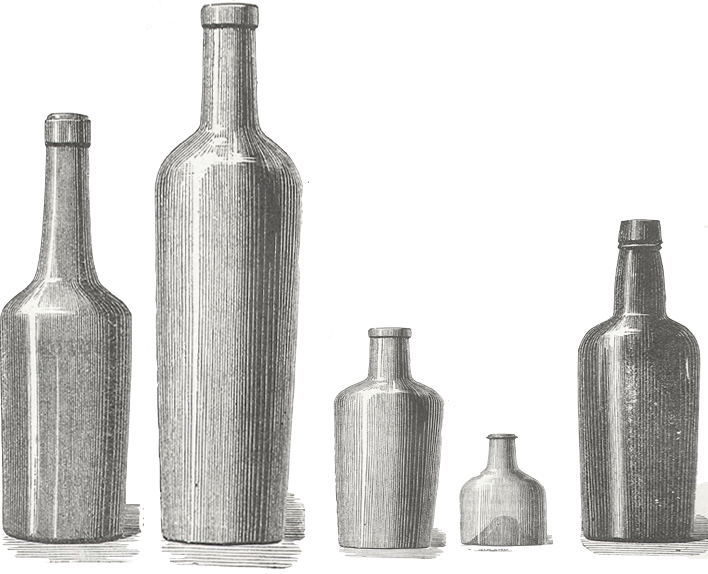
\includegraphics[width = 5cm]{img/messy_bottles.png}



\section*{Input}

The input consists of two lines.
On the first line, the number $n$ of bottles on the shelf, with $1\leq n\leq 100\,000$.
On the second line, $n$ integers, separated by space, giving the height (in nanometers) of each bottle from left to right.
Each height is an integer between $1$ and $10^9$.

\section*{Output}

Output a single integer: the messiness of the shelf.
Note that this number can be quite large, but no larger than $\binom{n}{3}$, which is bounded by $2 \times 10^{14}$.

\section*{Scoring}

Your score depends on the length of the shelf that you can handle within the time limit.
You get one point for $n\leq 1\,000$, another for $n\leq 10\,000$, and yet another for $100\,000$. 
The maximum score is $3$~points.

